\documentclass{article}
\usepackage{preamble}
\usetikzlibrary{3d}
\setlength\parskip{5pt}

\makenoidxglossaries

\newglossaryentry{declination}{
    name=declination (DEC),
    description={the angular distance north or south of the celestial equator},
}

\newglossaryentry{lunar eclipse}{
    name=lunar eclipse,
    description={an eclipse of the Moon, in which the Moon moves into the shadow of Earth; lunar eclipses can occur only at the time of full moon}
}

\newglossaryentry{right ascension}{
    name=right ascension (RA),
    description={the coordinate for measuring the east-west positions of celestial bodies; the angle measured eastward along the celestial equator from the vernal equinox to the hour circle passing through a body}
}

\newglossaryentry{solar eclipse}{
    name=solar eclipse,
    description={an eclipse of the Sun by the Moon, caused by the passage of the Moon in front of the Sun; solar eclipses can occur only at the time of the new moon}
}

\newglossaryentry{international date line}{
    name=international date line,
    description={an arbitrary line on the surface of Earth near longitude \SI{180}{\degree} across which the date changes by one day}
}

\newglossaryentry{phases}{
    name={phases of the Moon},
    description={the different appearance of light and dark on the Moon as seen from Earth during its monthly cycle, from new moon to full moon and back to new moon}
}

\newglossaryentry{meridian}{
    name=meridian,
    description={a great circle on the terrestrial or celestial sphere that passes through the north celestial pole and the zenith; a great circle that passe through the north and south cardinal directions and divides the sky in half}
}

\newglossaryentry{solar day}{
    name=solar day,
    description={Earth's rotation period as defined by the position of the Sun in the sky; the time between successive passages of the Sun through the meridian}
}

\newglossaryentry{season}{
    name=season,
    description={one of four stages of climate variation that Earth undergoes throughout a solar year as Earth revolves around the Sun}
}


\begin{document}

Astronomy \hfill Lecture Notes \hfill Chapter 4: {\small Earth, Moon \& Sky}
\vspace{1em}

% \section*{4.1 Earth and Sky}

% Locations on Earth are specified by latitude and longitude coordinates

% (Similar coordinate system exists for celestial sphere)



% \gls{meridian}: a great circle on the terrestrial or celestial sphere that passes through the North and South poles

% Go outside, point north, point south, and find the meridian. 



% \begin{figure}[h!]
%     \centering
% \begin{tikzpicture}[scale=1,every node/.style={minimum size=1cm}]
% \def\R{2.5} % sphere radius
% \def\angEl{10} % elevation angle
% \def\angBeta{25} % latitude of point P and Q

% \node at (\R*0.1,-\R*0.3) {\textbf{S}};
% \pgfmathsetmacro\H{\R*cos(\angEl)} % distance to north pole
% \shade[ball color=white,path fading=fade inside] (0,0) circle (\R);
% \node[left] at (0.2,0.7) {\textbf{N}};
% \coordinate[mark coordinate] (O) at (0,0);

% \begin{scope}[rotate=90]
%     \DrawLatitudeCircleRedBack[\R]{0}
%     %\DrawLatitudeCircleRedBack[\R]{-\angBeta}      
% \end{scope}

% \DrawLatitudeCircle[\R]{0}
% \FillLatitudeCircle[\R]{0} % equator

% \begin{scope}[rotate=90]
%     \DrawLatitudeCircleRedFront[\R]{0}  
% \end{scope}

% \node[left] at (-\R*0.9,0) {\textbf{W}};
% \node[right] at (\R*0.9,0) {\textbf{E}};
% \node at (0,1.2*\R) {\textbf{Meridian}};

% \node at (0,0.1) {\Strichmaxerl[1.8]};
% \end{tikzpicture}
% \end{figure}


% \gls{declination}: angular distance north or south of celestial equator

% \gls{right ascension}: angular distance east or west of vernal equinox (Pisces)

\section*{Seasons}

Seasons: one of four climate stages of the year: spring, summer, fall, winter

Seasons NOT caused by changes in distance between Earth and Sun

Seasons caused by tilt of Earth's axis

As it rotates Sun, Earth tilted on axis by \SI{23.5}{\degree}

\framebox{\textbf{Link}} \textit{YouTube}: ``The Earths Tilt'' by \texttt{St Marys Science} (\href{https://youtu.be/e9MU4TouzII}{click here})



%%%%%%%%%%%%%%%%%%%%%%%%%%%%%%%%%%%%%%%%%%%%%%%%%%%%%
%%% DO NOT EDIT FIGURE 4.5. GO TO SOURCE CODE INSTEAD %%%
%%%%%%%%%%%%%%%%%%%%%%%%%%%%%%%%%%%%%%%%%%%%%%%%%%%%%
\begin{figure}[h!]
\centering
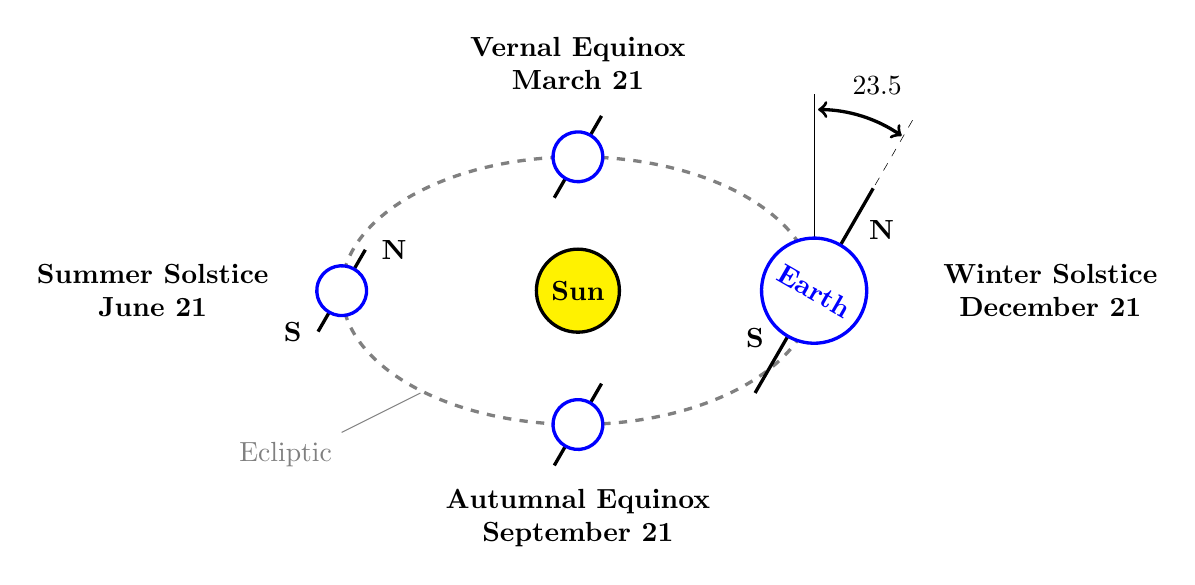
\begin{tikzpicture}	
\def\angTilt{30} % slightly above true 23.5 for emphasis
\def\a{3}
\def\b{1.7}
	
\draw[gray,very thick, dashed] (0,0) ellipse (\a cm and \b cm);

\draw[gray] (-2,-1.3) --++ (-1,-0.5) node[below left] {Ecliptic};

\draw (3,0) -- (3,2.5);

\draw[very thick,<->] (3.05,2.3) arc (90:55:1.85);
\node at (3.8,2.6) {\SI{23.5}{\degree}};

\draw[very thick,fill=yellow] (0,0) circle (15pt) node {\textbf{Sun}}; 

\begin{scope}[yshift=-\b cm,rotate=-\angTilt]
\draw[very thick] (0,0) -- (0,0.6);
\draw[very thick] (0,0) -- (0,-0.6);  
\draw[very thick,blue,fill=white] (0,0) circle (9pt);
\end{scope}

\begin{scope}[yshift=\b cm,rotate=-\angTilt]
\draw[very thick] (0,0) -- (0,0.6);
\draw[very thick] (0,0) -- (0,-0.6);  
\draw[very thick,blue,fill=white] (0,0) circle (9pt);
\end{scope}

\begin{scope}[xshift=-\a cm,rotate=-\angTilt]
\draw[very thick] (0,0) -- (0,0.6) node[right=2pt] {\textbf{N}};
\draw[very thick] (0,0) -- (0,-0.6) node[left=2pt] {\textbf{S}};  
\draw[very thick,blue,fill=white] (0,0) circle (9pt);
\end{scope}

\begin{scope}[xshift=\a cm, rotate=-\angTilt]
\draw[very thin,dashed] (0,2.5) -- (0,0);
\draw[very thick] (0,0) -- (0,1.5) node[xshift=3, yshift=-15] {\textbf{N}};
\draw[very thick] (0,0) -- (0,-1.5) node[yshift=20] {\textbf{S}};   
\draw[very thick,blue,fill=white] (0,0) circle (19pt) node {\rotatebox{-\angTilt}{\textbf{Earth}}};
\end{scope}

\node[align=center] at (2*\a,0) {\textbf{Winter Solstice}\\ \textbf{December 21}};
\node[align=center] at (-1.8*\a,0) {\textbf{Summer Solstice}\\ \textbf{June 21}};
\node[align=center] at (0,1.7*\b) {\textbf{Vernal Equinox}\\ \textbf{March 21}};
\node[align=center] at (0,-1.7*\b) {\textbf{Autumnal Equinox}\\ \textbf{September 21}};

\end{tikzpicture}
\end{figure}
%%%%%%%%%%%%%%%%%%%%%%%%%%%%%%%%%%%%%%%%%%%%%%%%%%%%%
%%% DO NOT EDIT FIGURE 4.5. GO TO SOURCE CODE INSTEAD %%%
%%%%%%%%%%%%%%%%%%%%%%%%%%%%%%%%%%%%%%%%%%%%%%%%%%%%%

%%%%%%%%%%%%%%%%%%%%%%%%%%%%%%%%%%%%%%%%%%%%%%%%%%%%%
%%% DO NOT EDIT FIGURE 4.7. GO TO SOURCE CODE INSTEAD %%%
%%%%%%%%%%%%%%%%%%%%%%%%%%%%%%%%%%%%%%%%%%%%%%%%%%%%%

In Summer, Texas tilted TOWARDS Sun $\Rightarrow$ Texas gets HOTTER

In December, Texas tilted AWAY FROM Sun $\Rightarrow$ Texas gets COLDER

In Sep and March, Earth's hemispheres get equal sunlight

\hgraydashline

Two reasons why North hemisphere is warmer in summer (June)

1) Sunlight hits surface at more direct angle $\Rightarrow$ more intense, effective sunlight (Gizmos Lab)

2) Days are longer

In June, Sun is north of celestial equator; spends more time (15 hours) northern countries

More time = longer warming time

In December, opposite case is true

On June 21 (Summer Solstice, 1st day of summer), Sun shines MOST directly at latitude \SI{23}{\degree} north of equator 

To a person at \SI{23}{\degree} N (e.g., Hawaii) on Jun 21, Sun directly overhead (at zenith) at noon.

Latitude \SI{23}{\degree} N called ``Tropic of Cancer''

Tropic of Cancer latitude same as Earth's tilt (\SI{23.5}{\degree}) 


In Summer, North Pole is continuously illuminated by the Sun; all places within \SI{23}{\degree} of the pole have sunshine for 24 hours

%See camera on 9/28/2022 for lecture notes

% Latitude at \SI{23}{\degree} below North Pole (\SI{67}{\degree} N) called Article Circle

% Southern Hemisphere has Tropic of Capricorn and Antarctic Circle for similar reasons

% Many early cultures scheduled special events around the summer solstice to celebrate the longest days and thank their gods for making the weather warm.

% Cultures north of equator celebrate around December 21 to cope with the depressing lack of sunlight and cold temperatures

% Huddle with family and friends

% Share food and drink

% Perform rituals asking gods to return light and heat; turn cycle of seasons around

% The points where the Sun crosses the celestial equator are called the vernal (spring) and autumnal (fall) equinoxes.








\clearpage
\begin{figure}[h!]
\begin{tikzpicture}[scale=1,every node/.style={minimum size=1cm}]

\def\R{2.5} % sphere radius
\def\angEl{10} % elevation angle
\def\angBeta{25} % latitude of point P and Q


\pgfmathsetmacro\H{\R*cos(\angEl)} % distance to north pole
\shade[ball color=white,path fading=fade inside] (0,0) circle (\R); 
\coordinate[mark coordinate] (O) at (0,0);

\node[left] at (0.2,0.7) {\small \textbf{E}};

\begin{scope}[rotate=45]
    \DrawLatitudeCircleRedBack[\R]{\angBeta}
    \DrawLatitudeCircleBack[\R]{0}
\end{scope}

\draw (-\H*0.8,\H*0.8) --++ (0,\H*0.2) node[above=-10pt]{North celestial pole};

\DrawLatitudeCircle[\R]{0}
\FillLatitudeCircle[\R]{0} % equator

\begin{scope}[rotate=45]
    \draw[very thick] (0,\H*1.25) -- (0,\H) (0,-\H) -- (0,-\H*1.25);
    \draw[dashed,very thin] (0,\H) -- (0,0) (0,-0.3*\H) -- (0,-\H);
    \DrawLatitudeCircleRedFront[\R]{\angBeta}
    \DrawLatitudeCircleFront[\R]{0}
    \fill[red] (0.8,1.4) circle (4pt);
\end{scope}

\draw (-\H*0.5,-\H*0.65) --++ (-\H*0.2,-\H*0.3) node[below=-6pt] {Celestial equator};
\node[left] at (-\R*0.9,0) {\textbf{N}};
\node[right] at (\R*0.9,0) {\textbf{S}};
\node at (\R*0.1,-\R*0.3) {\small \textbf{W}};
    
\draw[thick] (\H*0.32,\H*0.8) --++ (\H*0.3,\H*0.2) node[align=left,anchor=south west] {Sun's path\\ June 21};

\node at (0,0.1) {\Strichmaxerl[1.8]};
\end{tikzpicture}%
\hfill
\begin{tikzpicture}[scale=1,every node/.style={minimum size=1cm}]
\def\R{2.5} % sphere radius
\def\angEl{10} % elevation angle
\def\angBeta{25} % latitude of point P and Q

\node at (\R*0.1,-\R*0.3) {\small \textbf{W}};
\pgfmathsetmacro\H{\R*cos(\angEl)} % distance to north pole
\shade[ball color=white,path fading=fade inside] (0,0) circle (\R);
\coordinate[mark coordinate] (O) at (0,0);
\node[left] at (0.2,0.7) {\small \textbf{E}};
\begin{scope}[rotate=45]
    \DrawLatitudeCircleRedBack[\R]{0}
    %\DrawLatitudeCircleRedBack[\R]{-\angBeta}        
\end{scope}

\draw (-\H*0.8,\H*0.8) --++ (0,\H*0.2) node[above=-10pt]{North celestial pole};
\DrawLatitudeCircle[\R]{0}
\FillLatitudeCircle[\R]{0} % equator

\begin{scope}[rotate=45]
    \draw[very thick] (0,\H*1.25) -- (0,\H) (0,-\H) -- (0,-\H*1.25);
    \draw[dashed,very thin] (0,\H) -- (0,0) (0,-0.3*\H) -- (0,-\H);
    \DrawLatitudeCircleRedFront[\R]{0}
    %\DrawLatitudeCircleRedFront[\R]{-\angBeta}        
\end{scope}

\draw (-\H*0.5,-\H*0.65) --++ (-\H*0.2,-\H*0.3) node[below=-6pt] {Celestial equator};
\node[left] at (-\R*0.9,0) {\textbf{N}};
\node[right] at (\R*0.9,0) {\textbf{S}};
\draw[thick] (\H*0.7,\H*0.6) --++ (\H*0.3,\H*0.3) node[align=left,anchor=south west] {Sun's path\\ March 21\\ Sept.~21};
\fill[red] (0.8,1.3) circle (4pt);

\node at (0,0.1) {\Strichmaxerl[1.8]};
\end{tikzpicture}
\end{figure}


\begin{figure}[h!]
    \centering
\begin{tikzpicture}[scale=1,every node/.style={minimum size=1cm}]
\def\R{2.5} % sphere radius
\def\angEl{10} % elevation angle
\def\angBeta{25} % latitude of point P and Q

\node at (\R*0.1,-\R*0.3) {\small \textbf{W}};
\pgfmathsetmacro\H{\R*cos(\angEl)} % distance to north pole
\shade[ball color=white,path fading=fade inside] (0,0) circle (\R);
\coordinate[mark coordinate] (O) at (0,0);

\node[left] at (0.2,0.7) {\small \textbf{E}};

\begin{scope}[rotate=45]
    \DrawLatitudeCircleBack[\R]{0}
    \DrawLatitudeCircleRedBack[\R]{-\angBeta}        
\end{scope}

\draw (-\H*0.8,\H*0.8) --++ (0,\H*0.2) node[above=-10pt]{North celestial pole};
\DrawLatitudeCircle[\R]{0}
\FillLatitudeCircle[\R]{0} % equator

\begin{scope}[rotate=45]
    \draw[very thick] (0,\H*1.25) -- (0,\H) (0,-\H) -- (0,-\H*1.25);
    \draw[dashed,very thin] (0,\H) -- (0,0) (0,-0.3*\H) -- (0,-\H);
    \DrawLatitudeCircleFront[\R]{0}
    \DrawLatitudeCircleRedFront[\R]{-\angBeta}        
\end{scope}

\draw (-\H*0.5,-\H*0.65) --++ (-\H*0.2,-\H*0.3) node[below=-6pt] {Celestial equator};
\node[left] at (-\R*0.9,0) {\textbf{N}};
\node[right] at (\R*0.9,0) {\textbf{S}};
\draw[thick] (\H*0.85,\H*0.35) --++ (\H*0.1,\H*0.5) node[align=left,above] {Sun's path\\ December 21};
\fill[red] (1.8,0.7) circle (3pt);

\node at (0,0.1) {\Strichmaxerl[1.8]};
\end{tikzpicture}
\end{figure}
%%%%%%%%%%%%%%%%%%%%%%%%%%%%%%%%%%%%%%%%%%%%%%%%%%%%%
%%% DO NOT EDIT FIGURE 4.7. GO TO SOURCE CODE INSTEAD %%%
%%%%%%%%%%%%%%%%%%%%%%%%%%%%%%%%%%%%%%%%%%%%%%%%%%%%%

\gls{solar day}: time it takes Sun to go once around celestial sphere ($\approx \SI{24}{hours}$)

\gls{international date line}: Earth location at longitude \SI{180}{\degree} where the date changes

\clearpage

\section*{Phases and Motions of the Moon}

Moon does not shine like Sun; it reflects light from Sun

Moon orbits Earth once a month (every 27 days)

\gls{phases}: light and dark sides of Moon seen from Earth through the month

Phases we see depend on angle Moon makes with Sun

``New'' Moon is when Moon is in same direction as Sun

We see nothing of bright side; we only see dark side

One or two days later, see thin crescent

The next phases are first quarter and waxing Gibbous

Full moon is when moon is opposite direction of Sun; side illuminated by Sun is also facing us

\begin{figure}[h!]
    \centering
    \includegraphics[width=4in]{Figures/Figure4.14.jpg}
    \caption{Caption}
    \label{fig:my_label}
\end{figure}


\clearpage

\section*{Eclipses of the Sun and Moon}

Sun is 400 times larger in diameter than Moon; also 400 times farther away

Leads to Sun and Moon being same apparent size on sky

Leads to sometimes Moon getting ``in front'' of Sun

\gls{solar eclipse}: rare, local event where Moon blocks the sunlight

During solar eclipse, Earth enters Moon's shadow (umbra and penumbra)

Can solar eclipses happen every month? No b/c Moon orbit tilted \SI{5}{\degree} from ecliptic

Max solar eclipse time about 7 minutes

During solar eclipse, can see Sun's outer atmosphere (called corona)


\begin{figure}[h!]
    \centering
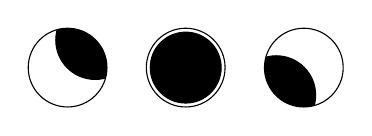
\begin{tikzpicture}
    \draw (0,0) circle (0.5cm);
    \begin{scope}
        \clip (0,0) circle (0.5cm);
        \draw[fill=black] (0.35,0.35) circle (0.5cm);
    \end{scope}

    \draw (1.5,0) circle (0.5cm);
    \draw[fill=black] (1.5,0) circle (0.45cm);

    \draw (3,0) circle (0.5cm);
    \begin{scope}
        \clip (3,0) circle (0.5cm);
        \draw[fill=black] (2.65,-0.35) circle (0.5cm);
    \end{scope}

\end{tikzpicture}
\end{figure}


\hgraydashline

\framebox{\textbf{Demo}} Students hold flashlight (Sun) and Moon models. Teacher holds Earth model to block sunlight on lunar surface. Emphasize that in reality Moon does the moving, not Earth (demo is easier to conduct by holding Earth). 

Sometimes Moon enters Earth's shadow

\gls{lunar eclipse}: rare event where Earth blocks sunlight on Moon's surface

Lunar eclipse visible to EVERYONE (unlike solar eclipse)

Lunar eclipse last longer (approx 3.5 hours) than solar eclipse b/c Earth's BIG shadow

Next Texas lunar eclipse: November 8, 2022

L eclipse called ``Blood Moon''

Red/orange color of Moon due to sunlight passing through Earth's atmosphere

Lunar eclipse NOT dangerous to look at

\framebox{\textbf{Practice}} If you're standing on the Moon during a lunar eclipse, what would your sky look like? What would the ground look like?

\framebox{\textbf{Link}} \textit{YouTube}: ``Lunar Eclipse 101'' by \texttt{National Geographic} (\href{https://youtu.be/VW2xRR75lKE}{click here})





\clearpage

\printnoidxglossaries
\end{document}